\section{eo\-Real\-Vector\-Bounds Class Reference}
\label{classeo_real_vector_bounds}\index{eoRealVectorBounds@{eoRealVectorBounds}}
Now a derived class, for parser reading It holds some of the bounds (and destroy them when dying).  


{\tt \#include $<$eo\-Real\-Vector\-Bounds.h$>$}

Inheritance diagram for eo\-Real\-Vector\-Bounds::\begin{figure}[H]
\begin{center}
\leavevmode
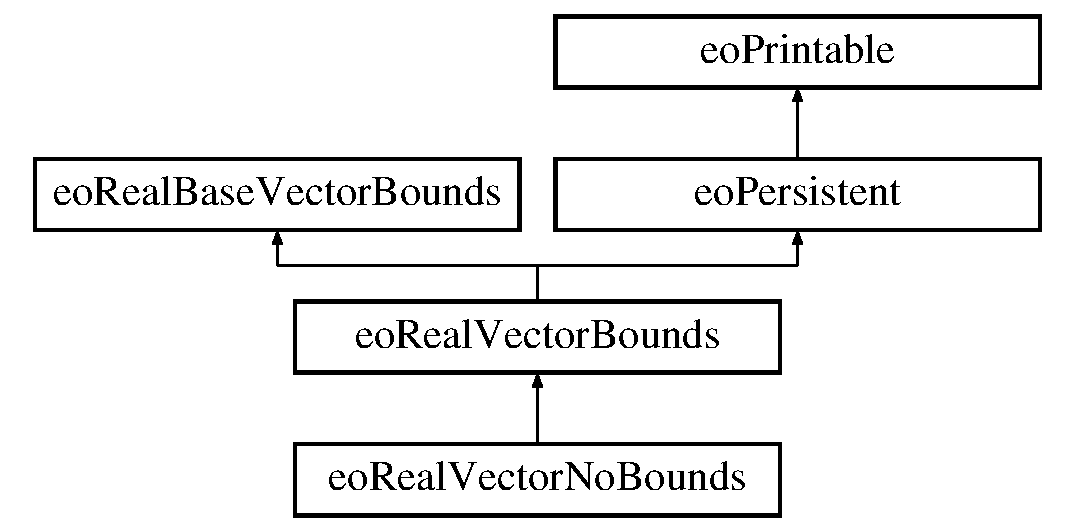
\includegraphics[height=4cm]{classeo_real_vector_bounds}
\end{center}
\end{figure}
\subsection*{Public Member Functions}
\begin{CompactItemize}
\item 
{\bf eo\-Real\-Vector\-Bounds} ()\label{classeo_real_vector_bounds_a0}

\begin{CompactList}\small\item\em Default Ctor will call base class default ctor. \item\end{CompactList}\item 
{\bf eo\-Real\-Vector\-Bounds} (unsigned \_\-dim, {\bf eo\-Real\-Bounds} \&\_\-bounds)\label{classeo_real_vector_bounds_a1}

\begin{CompactList}\small\item\em Ctor: same bounds for everybody, given as an {\bf eo\-Real\-Bounds}{\rm (p.\,\pageref{classeo_real_bounds})}. \item\end{CompactList}\item 
{\bf eo\-Real\-Vector\-Bounds} ({\bf eo\-Real\-Bounds} \&\_\-xbounds, {\bf eo\-Real\-Bounds} \&\_\-ybounds)\label{classeo_real_vector_bounds_a2}

\begin{CompactList}\small\item\em Ctor, particular case of dim-2. \item\end{CompactList}\item 
{\bf eo\-Real\-Vector\-Bounds} (unsigned \_\-dim, double \_\-min, double \_\-max)\label{classeo_real_vector_bounds_a3}

\begin{CompactList}\small\item\em Simple bounds = minimum and maximum (allowed). \item\end{CompactList}\item 
{\bf eo\-Real\-Vector\-Bounds} (std::vector$<$ double $>$ \_\-min, std::vector$<$ double $>$ \_\-max)\label{classeo_real_vector_bounds_a4}

\begin{CompactList}\small\item\em Ctor: different bounds for different variables, std::vectors of double. \item\end{CompactList}\item 
{\bf eo\-Real\-Vector\-Bounds} (std::string \_\-s)\label{classeo_real_vector_bounds_a5}

\begin{CompactList}\small\item\em Ctor from a std::string and don't worry, the {\bf read\-From(std::string)}{\rm (p.\,\pageref{classeo_real_vector_bounds_a8})} starts by setting everything to 0! \item\end{CompactList}\item 
virtual {\bf $\sim$eo\-Real\-Vector\-Bounds} ()\label{classeo_real_vector_bounds_a6}

\begin{CompactList}\small\item\em Dtor: destroy all owned\-Bounds - BUG ??? \item\end{CompactList}\item 
virtual void {\bf read\-From} (std::istream \&\_\-is)
\begin{CompactList}\small\item\em Read object from a stream only calls the {\bf read\-From(std::string)}{\rm (p.\,\pageref{classeo_real_vector_bounds_a8})} - for param reading. \item\end{CompactList}\item 
virtual void {\bf read\-From} (std::string \_\-s)
\begin{CompactList}\small\item\em Read object from a std::string. \item\end{CompactList}\item 
virtual void {\bf print\-On} (std::ostream \&\_\-os) const \label{classeo_real_vector_bounds_a9}

\begin{CompactList}\small\item\em overload print\-On method to save space \item\end{CompactList}\item 
void {\bf adjust\_\-size} (unsigned \_\-dim)\label{classeo_real_vector_bounds_a10}

\begin{CompactList}\small\item\em Eventually increases the size by duplicating last bound. \item\end{CompactList}\item 
{\bf eo\-Real\-Vector\-Bounds} (const {\bf eo\-Real\-Vector\-Bounds} \&)\label{classeo_real_vector_bounds_a11}

\begin{CompactList}\small\item\em need to rewrite copy ctor and assignement operator because of owned\-Bounds \item\end{CompactList}\end{CompactItemize}
\subsection*{Private Member Functions}
\begin{CompactItemize}
\item 
{\bf eo\-Real\-Vector\-Bounds} \& {\bf operator=} (const {\bf eo\-Real\-Vector\-Bounds} \&)\label{classeo_real_vector_bounds_d0}

\end{CompactItemize}
\subsection*{Private Attributes}
\begin{CompactItemize}
\item 
std::vector$<$ unsigned int $>$ {\bf factor}\label{classeo_real_vector_bounds_r0}

\item 
std::vector$<$ {\bf eo\-Real\-Bounds} $\ast$ $>$ {\bf owned\-Bounds}\label{classeo_real_vector_bounds_r1}

\end{CompactItemize}


\subsection{Detailed Description}
Now a derived class, for parser reading It holds some of the bounds (and destroy them when dying). 



Definition at line 228 of file eo\-Real\-Vector\-Bounds.h.

\subsection{Member Function Documentation}
\index{eoRealVectorBounds@{eo\-Real\-Vector\-Bounds}!readFrom@{readFrom}}
\index{readFrom@{readFrom}!eoRealVectorBounds@{eo\-Real\-Vector\-Bounds}}
\subsubsection{\setlength{\rightskip}{0pt plus 5cm}void eo\-Real\-Vector\-Bounds::read\-From (std::istream \& {\em \_\-is})\hspace{0.3cm}{\tt  [virtual]}}\label{classeo_real_vector_bounds_a7}


Read object from a stream only calls the {\bf read\-From(std::string)}{\rm (p.\,\pageref{classeo_real_vector_bounds_a8})} - for param reading. 

\begin{Desc}
\item[Parameters:]
\begin{description}
\item[{\em \_\-is}]A std::istream. \end{description}
\end{Desc}


Implements {\bf eo\-Persistent} {\rm (p.\,\pageref{classeo_persistent_a1})}.

Definition at line 65 of file eo\-Real\-Bounds.cpp.

Referenced by eo\-Real\-Vector\-Bounds().\index{eoRealVectorBounds@{eo\-Real\-Vector\-Bounds}!readFrom@{readFrom}}
\index{readFrom@{readFrom}!eoRealVectorBounds@{eo\-Real\-Vector\-Bounds}}
\subsubsection{\setlength{\rightskip}{0pt plus 5cm}void eo\-Real\-Vector\-Bounds::read\-From (std::string {\em \_\-s})\hspace{0.3cm}{\tt  [virtual]}}\label{classeo_real_vector_bounds_a8}


Read object from a std::string. 

\begin{Desc}
\item[Parameters:]
\begin{description}
\item[{\em \_\-is}]A std::istream. \end{description}
\end{Desc}


Definition at line 73 of file eo\-Real\-Bounds.cpp.

References adjust\_\-size().

The documentation for this class was generated from the following files:\begin{CompactItemize}
\item 
eo\-Real\-Vector\-Bounds.h\item 
eo\-Real\-Bounds.cpp\end{CompactItemize}
